\section{Results}
\label{sec:results}

\subsection{The budget has to bite before anything happens}
\label{sec:adequacy}
On the development split the compactor loses essentially nothing at the budgets it would normally run
under: retention at $k{=}10$ is \RetentionBThreeHundred{} at a 300-word budget and
\RetentionBSixHundred{} at 600. The prespecified adequacy condition --- retention at least 10
percentage points (pp) below the append-only access ceiling and inside $[0.10,0.90]$ --- is met only
at \BudgetB{} words, where retention is \RetentionOOne{} against a ceiling of \RetentionOSeven{}.
That budget was frozen with every other operating choice before any confirmatory family was touched.
This already answers the counter-evidence that strong models relay atomic facts losslessly
\citep{faithful2026}: they do, until the budget forces a choice.

\subsection{C1: making the same value expected does not help it survive}
\label{sec:c1}
\textsc{E-Shift} holds the target sentence and its value fixed and changes only a value-free
description of the work the user does. On \EShiftNFam{} eligible families (\EShiftNBlocks{} arm-paired
seed blocks) the frame shifts the compactor's elicited prior by \ShiftMeanConf{} log-odds on the
independent estimation half, in the predicted direction for \ShiftDirectionCountConf{} of them.
Survival does not follow. The mean paired difference is \EShiftMean{}~pp
(95\% CI [\EShiftCIlo{}, \EShiftCIhi{}]), so a benefit larger than about \ConeUpper{}~pp is ruled
out for this manipulation (Figure~\ref{fig:eshift}). The intention-to-treat analysis over all
prespecified families is identical (every prespecified family passed the eligibility screen), and the
secondary endpoint --- the originally preregistered binary retention at $k{=}10$ --- gives the same
picture. The \textsc{Copy-Rand} frame control, which cannot condition on the frame at all, differs by
\FrameControlMean{}~pp and is equivalent to zero within $\pm5$~pp, so the null is not an artifact of
the frame text occupying space in the seeding session.

\paragraph{What this does and does not establish.} The frozen rule returns
\textbf{\EShiftDecision{}} only because amendment~A1 replaced the originally preregistered $\pm8$~pp
margin with the design's minimum detectable effect, $\pm$\SESOI{}~pp, after the development power
analysis showed between-family heterogeneity put $8$~pp out of reach (power $0.32$; $0.80$ would need
roughly $60$ eligible families, not \EShiftNFam{}). We therefore do \emph{not} claim equivalence at
the margin we first chose. The defensible statement is one-sided: the predicted positive effect is
absent, and effects above \ConeUpper{}~pp in the predicted direction are excluded. The conclusion
does not depend on which judge is believed (\ConeJudgeOne{} and \ConeJudgeTwo{}~pp under each alone),
nor on the \EShiftUnresRate{} of \textsc{e-shift} cases left unresolved: resolving them all in the
least favourable direction gives \ConeWorstAgainst{}~pp, and in the most favourable
\ConeWorstFor{}~pp.

If anything the estimate runs the wrong way, and the next subsection gives a reason to take that
seriously rather than as noise.

\subsection{Our own manipulation is not clean, and we say how}
\label{sec:parity}
A context that changes what the compactor expects can change other things too. We asked the two blind
judges, with the target's value masked, how important, authoritative and relevant the target looks
under each frame. They differ: the expected-value frame is rated \ParityImp{} lower on importance
(95\% CI [\ParityImpLo{}, \ParityImpHi{}], 1--5 scale) and \ParityAuth{} lower on authority (95\%
CI [\ParityAuthLo{}, \ParityAuthHi{}]); relevance is inconclusive.

A frame that makes the target look \emph{less} important would depress its retention, which is
exactly the sign we observe. \textsc{E-Shift} therefore estimates an \emph{expectation-shifting
context manipulation}, not prior-fit in isolation, and its small negative estimate is plausibly a
perceived-importance effect rather than evidence that surprise \emph{helps}. What survives is the
one-sided exclusion: a manipulation raising the compactor's own elicited prior by \ShiftMeanConf{}
log-odds, in the predicted direction for \ShiftDirectionCountConf{} families, produces no retention
benefit above \ConeUpper{}~pp. The graded dose--response in \S\ref{sec:c2} has no frame at all, so
the two analyses fail in different ways and agree.

\begin{figure*}[t]
\centering
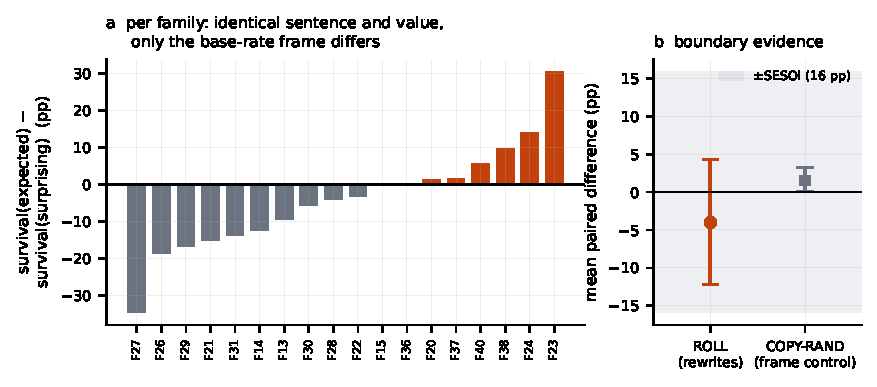
\includegraphics[width=0.78\textwidth]{figures/fig1_eshift.pdf}
\caption{\textbf{The causal test is null.} Each bar is one family, with the target sentence and its
value identical across arms. Right: the mean paired difference and the prespecified smallest effect
of interest, with the prior-blind frame control.}
\label{fig:eshift}
\end{figure*}

\subsection{C2--C3: no graded gradient either, under any operator}
\label{sec:c2}
The ecological version of the question gives the same answer. Regressing retention at $k{=}10$ on
within-family-centred measured surprise, with family fixed effects and a two-way crossed cluster
bootstrap over families and chain\,$\times$\,seed blocks, the slope under the rolling rewrite is
\SlopeOOne{}~pp per log-odds (95\% CI [\SlopeOOneCIlo{}, \SlopeOOneCIhi{}]), which is
\SlopeOOneIQR{}~pp across the interquartile surprise contrast of \IQRSurprise{} log-odds.
Retention by surprise tercile under the rolling rewrite is \LowOone{}\%, \MidOone{}\% and \HighOone{}\%
(Figure~\ref{fig:operators}a) --- flat, over a dose whose within-family range averages \BTRange{}
log-odds. The surprise\,$\times$\,operator interaction against the prior-blind control is
\InteractionPoint{}~pp (95\% CI [\InteractionCIlo{}, \InteractionCIhi{}]). The equivalence test on the
control slope does not clear its $\pm5$~pp margin, so we report that contrast as inconclusive rather
than as positive evidence of no difference; the point estimates in both arms are near zero.

Under the gatekeeping order frozen in advance, C1 did not pass, so C2 and C3 are reported as evidence
rather than as confirmed claims. They point the same way, and they do so through a design with no
frame and therefore no perceived-importance confound.

\subsection{Operators differ far more than surprise does (exploratory)}
\label{sec:operators}
What surprise does not explain, the choice of operator does
(Figure~\ref{fig:operators}b; all contrasts in Figure~\ref{fig:contrasts}). These contrasts were \emph{not}
preregistered and are not multiplicity-corrected; we report them as exploratory, and they are large
enough that the distinction matters little for the direction but should be kept in mind for the size.

Holding the model, the budget, the sessions and the stimuli fixed, reconstructing the memory from the
\emph{raw sessions} at every step retains \RetOfour{}\% at $k{=}10$, while rewriting from the
model's \emph{own previous memory} retains \RetOone{}\% --- a difference of \ContrastOfour{}~pp
(95\% CI [\ContrastOfourLo{}, \ContrastOfourHi{}]), stable under either judge alone
(\OfourJudgeOne{} and \OfourJudgeTwo{}~pp). By $k{=}20$ the gap is wider: \CurveOfourK{}\% against
\CurveOoneK{}\%.

The honest reading is \emph{reconstruction versus recursion}, not ``iteration is causal''.
\textsc{Src} differs from \textsc{Roll} in more than one way: repeated exposure, a longer and
differently composed input, and the ability to recover an item an earlier step happened to omit. What
we can defend is that recursive summaries \emph{accumulate} omissions, each step's loss being
permanent, while reconstruction resets that accumulation --- which is also why \S\ref{sec:adequacy}
and this subsection agree rather than conflict: the budget forces an omission at each step, recursion
makes it permanent. \textsc{Anchor} shows iteration alone is not sufficient for large loss: it is
just as recursive and retains \RetOfive{}\%, indistinguishable from \textsc{Src}
(\PairFourVsFive{}~pp, 95\% CI [\PairFourVsFiveLo{}, \PairFourVsFiveHi{}]).

\paragraph{Two prior-blind controls.} \textsc{Copy-Rand} keeps a fixed number of randomly chosen
source sentences, matched to \textsc{Roll} on \emph{retention} (\RetOthree{}\%) but not on capacity
(\WordsOthree{} words against \WordsOone{}). Its surprise slope is flat, which rules out the coder
and the regexes as a source of any gradient: a selector that cannot see the prior produces the same
flat profile through the same pipeline. The \emph{capacity}-matched version, packing random sentences
into \textsc{Roll}'s own budget, retains \RetOthreeW{}\% --- essentially nothing
(\PairThreeWVsOne{}~pp, 95\% CI [\PairThreeWVsOneLo{}, \PairThreeWVsOneHi{}]). At \textsc{Roll}'s
capacity random selection keeps no targets at all, so the compactor's selection is far better than
chance even as it loses a third of the items; that arm is too degenerate for a gradient test, which is
why both are reported.

Verbatim \emph{selection} by the model collapses to \RetOtwo{}\% by $k{=}10$: it keeps recent
conversational turns and lets the seeded facts go, a recency bias strong enough that this arm carries
no information about surprise and we do not interpret its slope.

\begin{figure*}[t]
\centering
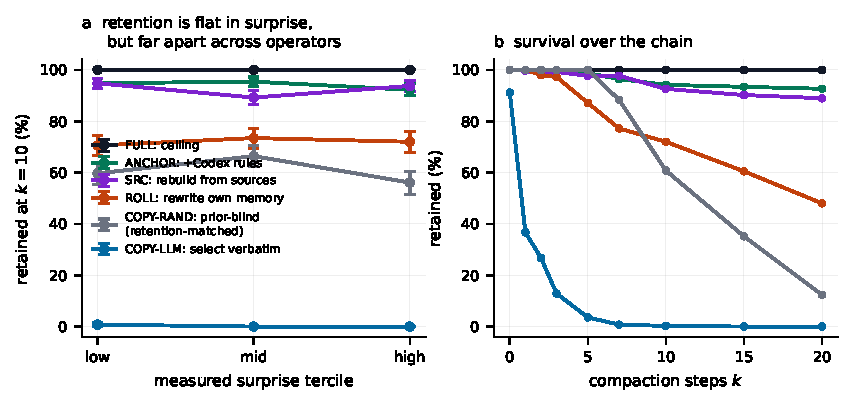
\includegraphics[width=0.78\textwidth]{figures/fig2_operators.pdf}
\caption{\textbf{Retention is flat in surprise but far apart across operators.} Left: retention at
$k{=}10$ by measured surprise tercile. Right: survival over the chain.}
\label{fig:operators}
\end{figure*}


\subsection{C5--C6: memory is deleted, not corrupted}
\label{sec:c6}
Across \NCodedCases{} coded item-checkpoints only \ChangedCount{} (\ChangedRate{}) are changes to a
different value, leaving \NChangedEvents{} usable events for the replacement-direction test --- far
too few to estimate a direction, which we report as a scoped null. The failure mode is deletion, and
deletion is close to absorbing (regeneration \RegenRate{}), which is why the formal account is about
survival rather than a stationary distribution. A value-level kernel fitted to the single step
$k{=}0\rightarrow1$ predicts the held-out $k{=}10$ distribution with total-variation distance
\KernelTVD{} against \KernelConstTVD{} for a constant-hazard baseline (Appendix~\ref{app:kernel}).

\subsection{C7: what to do about it}
\label{sec:c7}
The mitigation that works is the one already shipping. Adding the anti-drift rules from Codex's
memory-consolidation prompt to an otherwise identical rolling rewrite raises retention at $k{=}10$
from \RetOone{}\% to \RetOfive{}\%, a gain of \ContrastOfive{}~pp (95\% CI [\ContrastOfiveLo{},
\ContrastOfiveHi{}]) at no extra budget --- recovering almost the whole iteration penalty
(Figure~\ref{fig:mitigation}).

Surprise-pinning, the mitigation our theory predicted, shows \emph{no detected benefit}. Pinning the
highest-surprise items verbatim gives \ContrastOsix{}~pp relative to no mitigation (95\% CI
[\ContrastOsixLo{}, \ContrastOsixHi{}]) --- a negative point estimate whose interval still includes
zero, so we claim only that it fails to help, not that it is reliably harmful. The direct paired
contrast against token-matched \emph{random} pinning is \PairSixVsRandom{}~pp (95\% CI
[\PairSixVsRandomLo{}, \PairSixVsRandomHi{}]): choosing \emph{which} items to pin by surprise buys
nothing over choosing them at random. Pinning does do what it says --- pinned high-surprise items are
retained, which is why that arm's surprise slope is positive by construction --- but under a binding
budget the pinned text crowds out everything else and the memory as a whole is no better off.

\paragraph{A caveat on \textsc{Anchor}.} The anchoring rules make the model far more likely to
overshoot the word budget: \RetriesOfive{} regeneration attempts per trajectory against
\RetriesOone{} for the neutral prompt, and \TrimsOfive{} line-boundary trims against \TrimsOone{}.
\textsc{Anchor} therefore reaches its result through a noticeably different generation process, and it
stores \WordsOfive{} words against \WordsOone{}. Both differences work \emph{against} it --- trimming
deletes trailing content --- so the advantage is not an artifact of them, but the comparison is not
matched on protocol compliance and we do not treat the exact size as precise.

\begin{figure}[t]
\centering
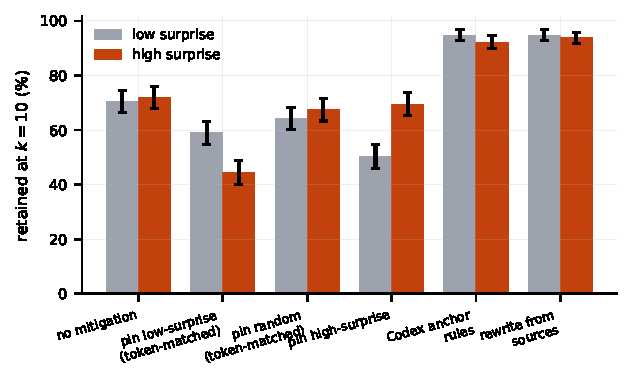
\includegraphics[width=0.86\linewidth]{figures/fig5_mitigation.pdf}
\caption{\textbf{The deployed anchoring prompt beats the theory-derived fix.} Retention at $k{=}10$
by surprise tercile. Pinning raises retention for the items it pins and lowers it overall.}
\label{fig:mitigation}
\end{figure}

\subsection{Robustness}
\label{sec:robust}
Appendix~\ref{app:robust} reports \emph{portability diagnostics}: the graded dose--response re-run on
a second strong family (Llama-3.3-70B), on a small local model (Qwen3-8B), and at temperature $0$.
Every slope interval contains zero. These are not repetitions of \textsc{E-Shift}, and they score each
model against the \emph{primary} compactor's measured prior rather than its own, so they are evidence
about the portability of the stimulus set rather than proof that each model ignores its own prior. The
weaker models lose far more content overall (\RetLlamaOone{}\% and \RetLocalOone{}\% at $k{=}10$
against \RetOone{}\%) and the reconstruction advantage reappears in both. The proxy caps temperature
at $1.0$, so $T>1$ could not be tested.

\subsection{A1: preferences, and the homogenisation that does not happen}
\label{sec:prefs}
User preferences are the case where drift-to-defaults is most often asserted, and in this constructed
set they show no sign of it. In stored memory, preferences that \emph{match} the model's own default
behaviour survive \PrefDefaultK{}\% of the time at $k{=}20$, while preferences that \emph{differ}
from it survive \PrefNonDefaultK{}\% (Figure~\ref{fig:prefs}a). Because default-matching and
non-default preferences are different items, the honest contrast subtracts the pre-existing gap at
$k{=}0$ (\PrefGapZero{}~pp) and clusters over the \PrefNFamilies{} preference families rather than
treating item-checkpoints as independent: the baseline-adjusted advantage of non-default content is
\PrefAdj{}~pp (95\% CI [\PrefAdjLo{}, \PrefAdjHi{}]). The surviving profile becomes more
distinctive, not less: the share of stored preferences that depart from the model's defaults rises
from \PrefShareZero{}\% at $k{=}0$ to \PrefShareK{}\% at $k{=}20$. Generalisation here is over
preference families; the eight profiles are controlled test cases, not a sample of people.

Separating storage from execution (Figure~\ref{fig:prefs}b), the model follows a stated preference
\PrefCondA{}\% of the time given raw instructions and \PrefCondC{}\% given nothing --- an execution
ceiling of \PrefExecLoss{}~pp unrelated to memory --- and memory costs a further
\PrefStorageLoss{}~pp by $k{=}20$. Neither loss is prior-shaped.

\begin{figure}[t]
\centering
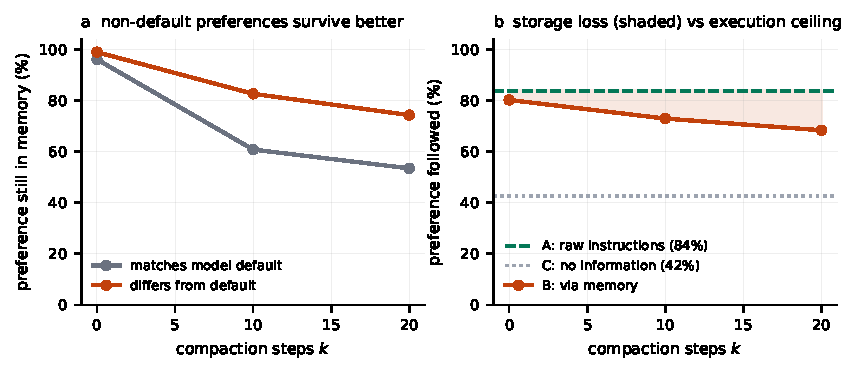
\includegraphics[width=0.96\linewidth]{figures/fig4_preferences.pdf}
\caption{\textbf{No preference homogenisation.} Left: stored-memory survival split by whether the
preference matches the model's own default. Right: storage loss against the execution ceiling.}
\label{fig:prefs}
\end{figure}
